\chapter{Model Characterization} \label{chapter-characterization}


\section{Base model of city and the production sector}
\newpage
 \subsection{The price. of output}
Underlying the housing analysis is an economic model of the city including firms and transportation.  The first question for an economist is likely to be is, "Does the system respond to an increase in demand for its export product in the expected ways?" 


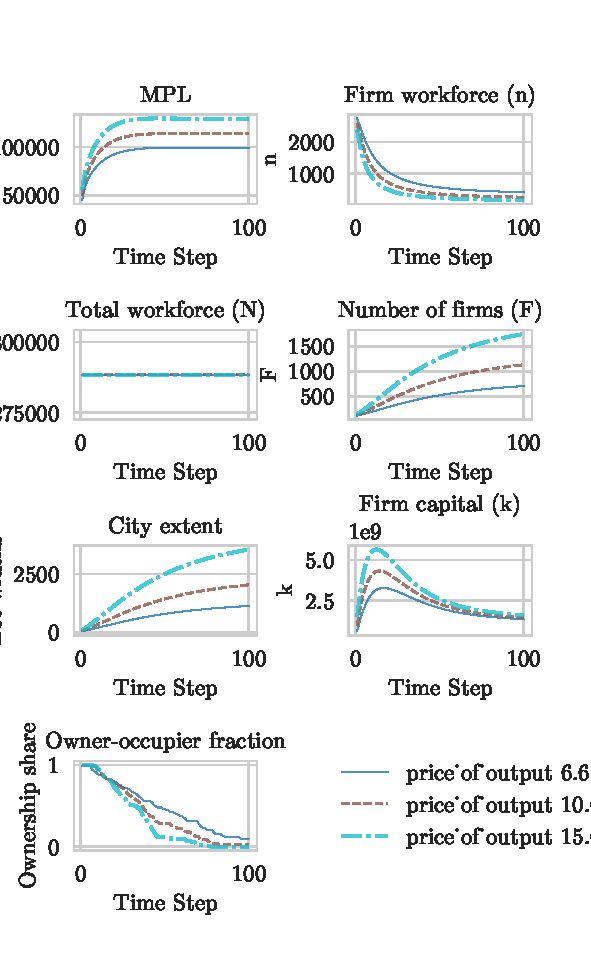
\includegraphics[scale=1]{fig/Analysis/price3.pdf}


 \subsection{Change junk}
\begin{figure}
  \centering
  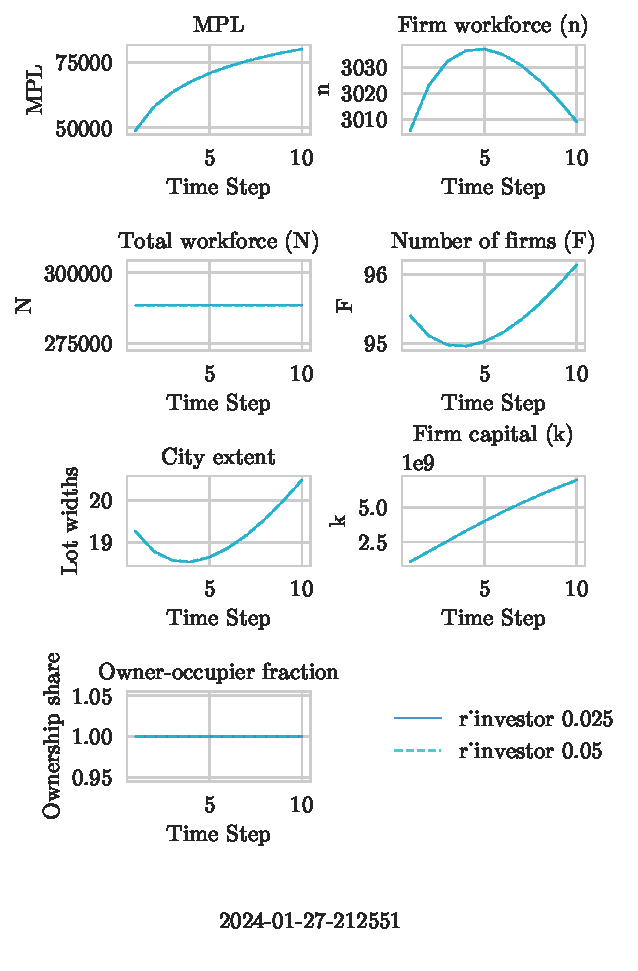
\includegraphics[width=.6\textwidth, clip, trim=0 20mm 0 0]{fig/plots/timeseries-plots-2024-01-27-212551.pdf}
  \caption{Your caption here.}
  \label{fig:your-label}
\end{figure}

 \subsection{Change Density}
 This experiment verifies that the labour-market/urban model that is the platform for the housing market analysis behaves exactly as expected when density changes. mpl, n, N, F, E, and k all rise. %Population rises with 

 The fraction owner-occupiers falls earlier with increasing density due to more rapid financialization and the potential rent capture increases, and not to changing housing form. It seems later entrants do not purchase. The transition is achieved in about two full generations in our model. The timing will be sensitive to the specific parameterization.
 

 \hspace*{-2cm}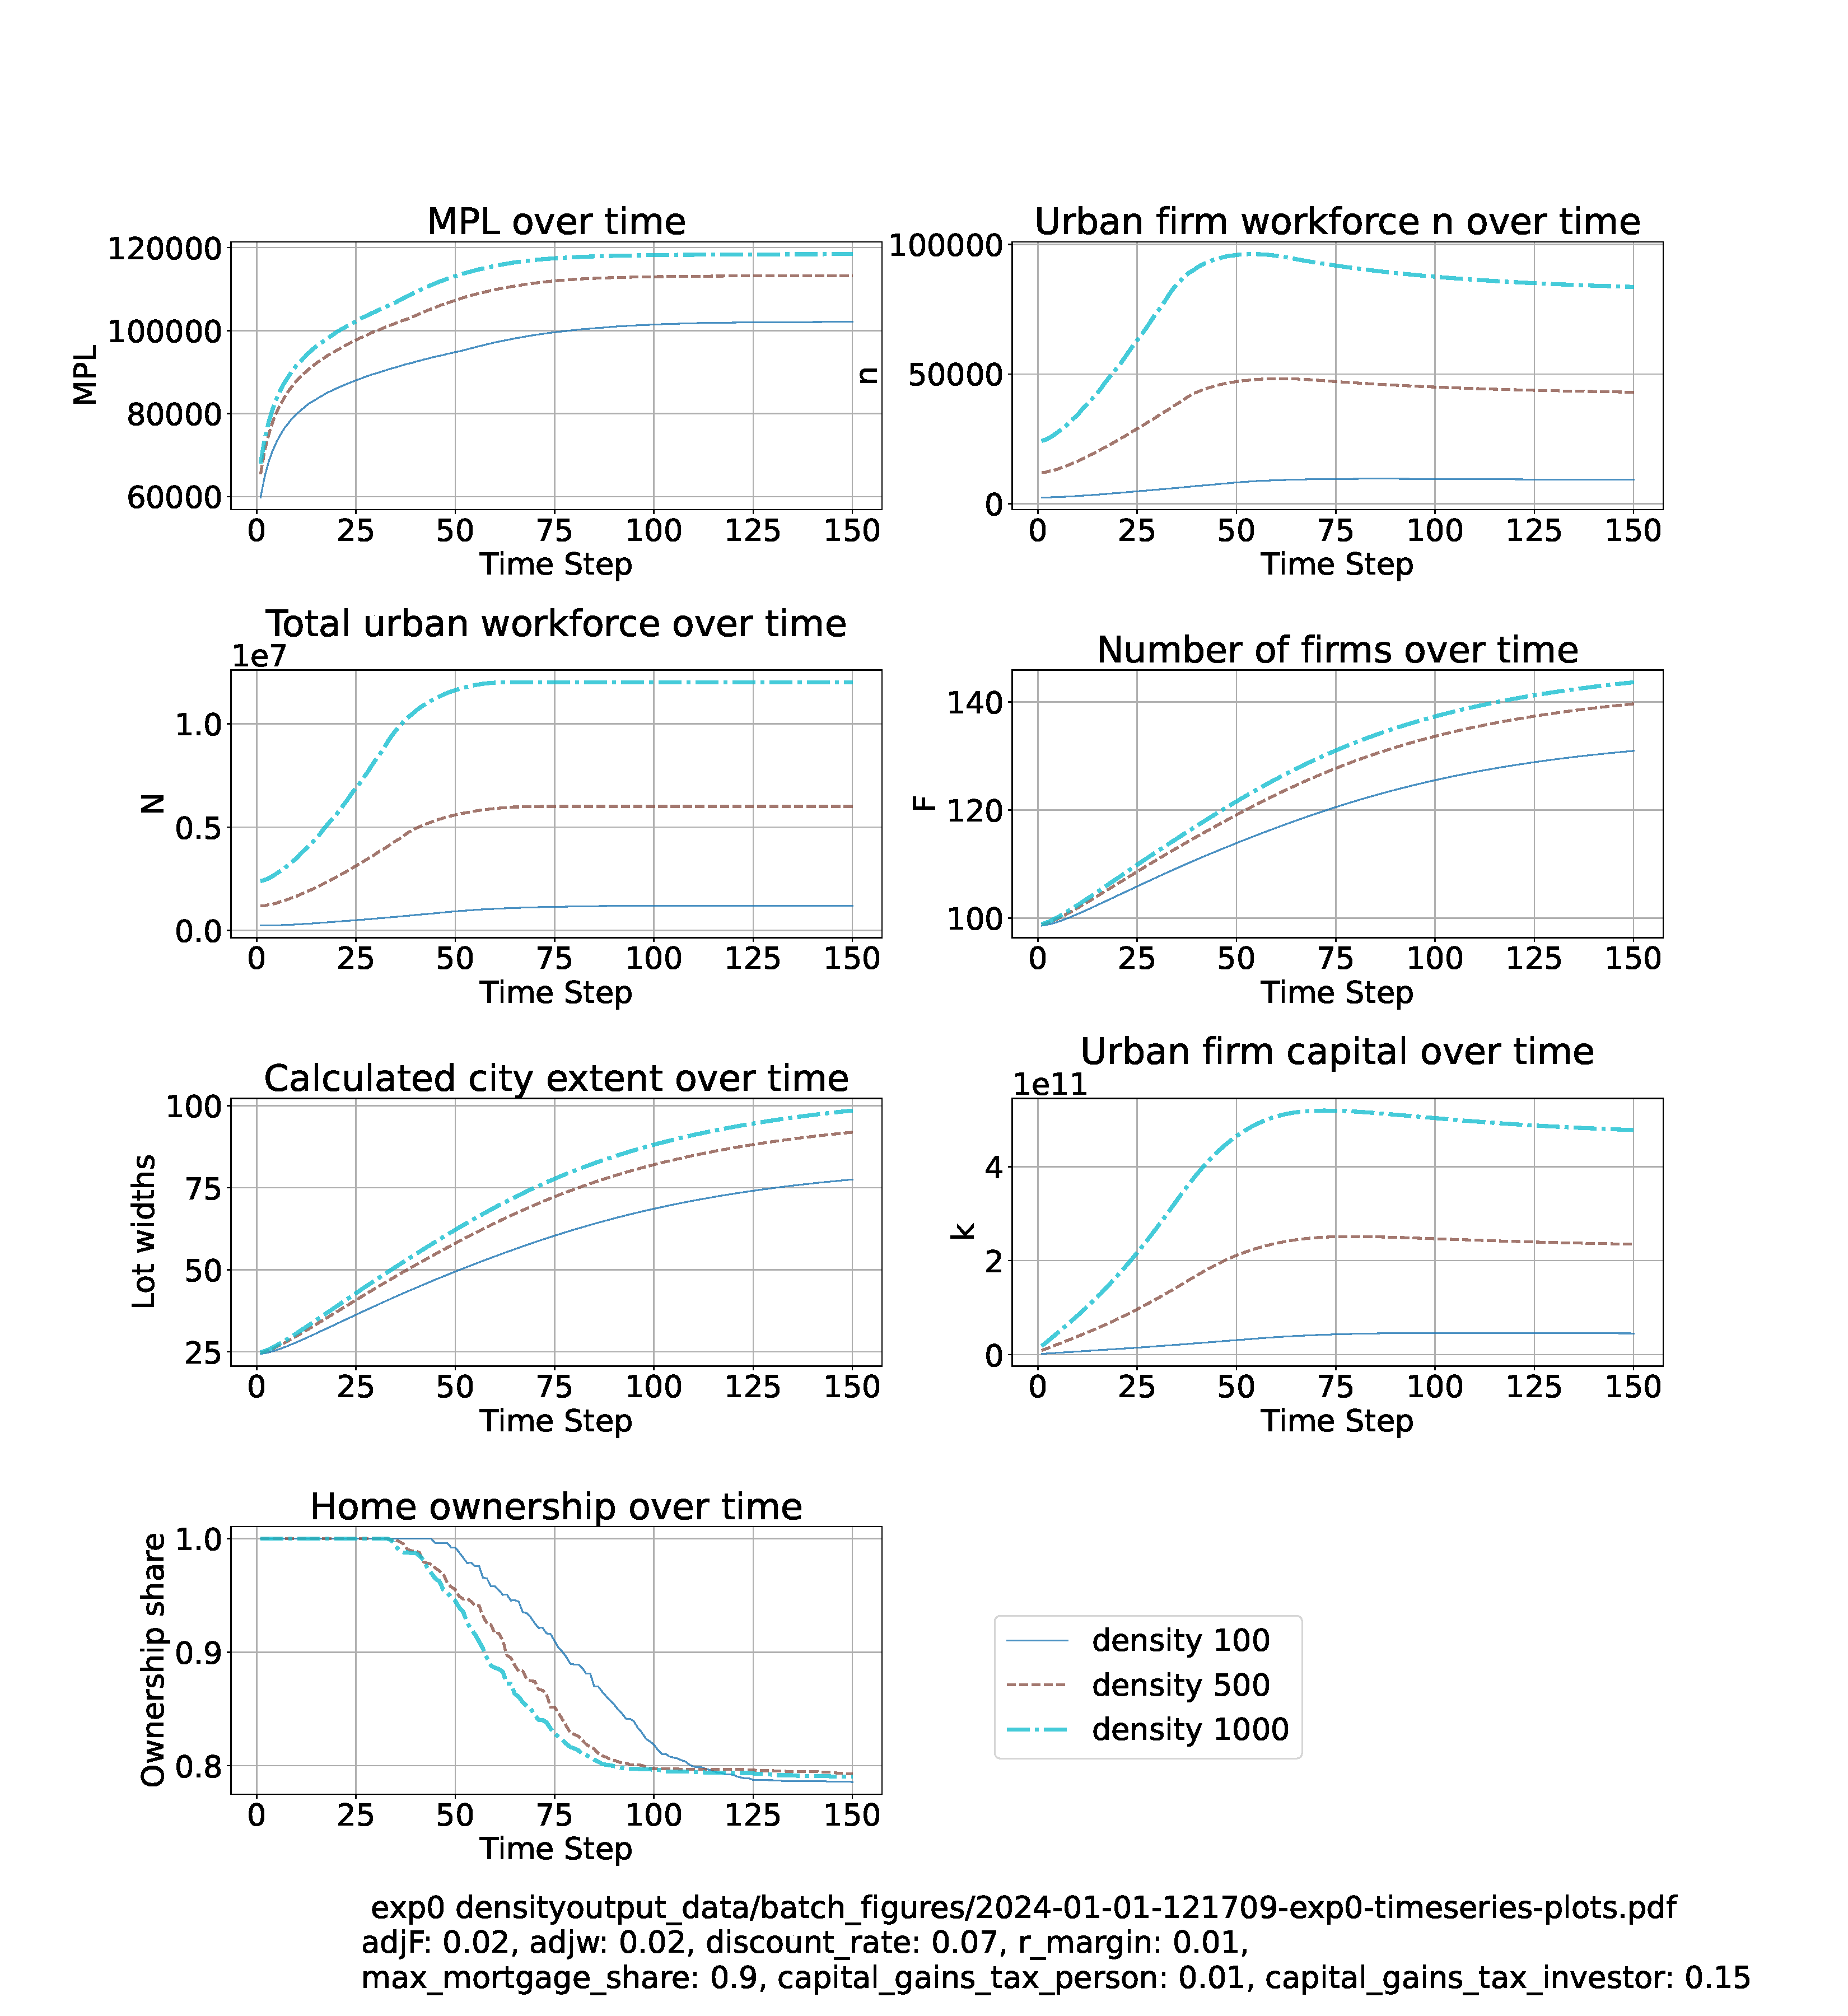
\includegraphics[trim= 1.5cm 3.65cm 2cm 4.0cm, clip, scale=.3]{fig/Analysis/Density-3-150.pdf}

\newpage %%%%%%%%%%%%%%%%%%%%%%%%%%%%%%%%%%

\subsection{High Gamma}
Very high levels of the agglomeration parameter Gamma are implausible. They drive up marginal productivity, causing very rapid growth, drive down firm size because the first worker is extremely productive but the MPL falls rapidly. Very small firms with high levels of capital multiply. Rapidly rising prices encourage investors while savings-limited owner-occupiers are squeezed out.

Higher agglomeration effects make land rents higher and increase the gains to investors, resulting in more rapid financialization of the housing stock.

%   we can check
 
% \begin{tabular}{|c|c||c|c||c|c|}
% mpl  & up   & n   & up & N   &  up \\
% F    & up   & E   &  up  &  k & up
% \end{tabular} 

 \hspace*{-2.5cm}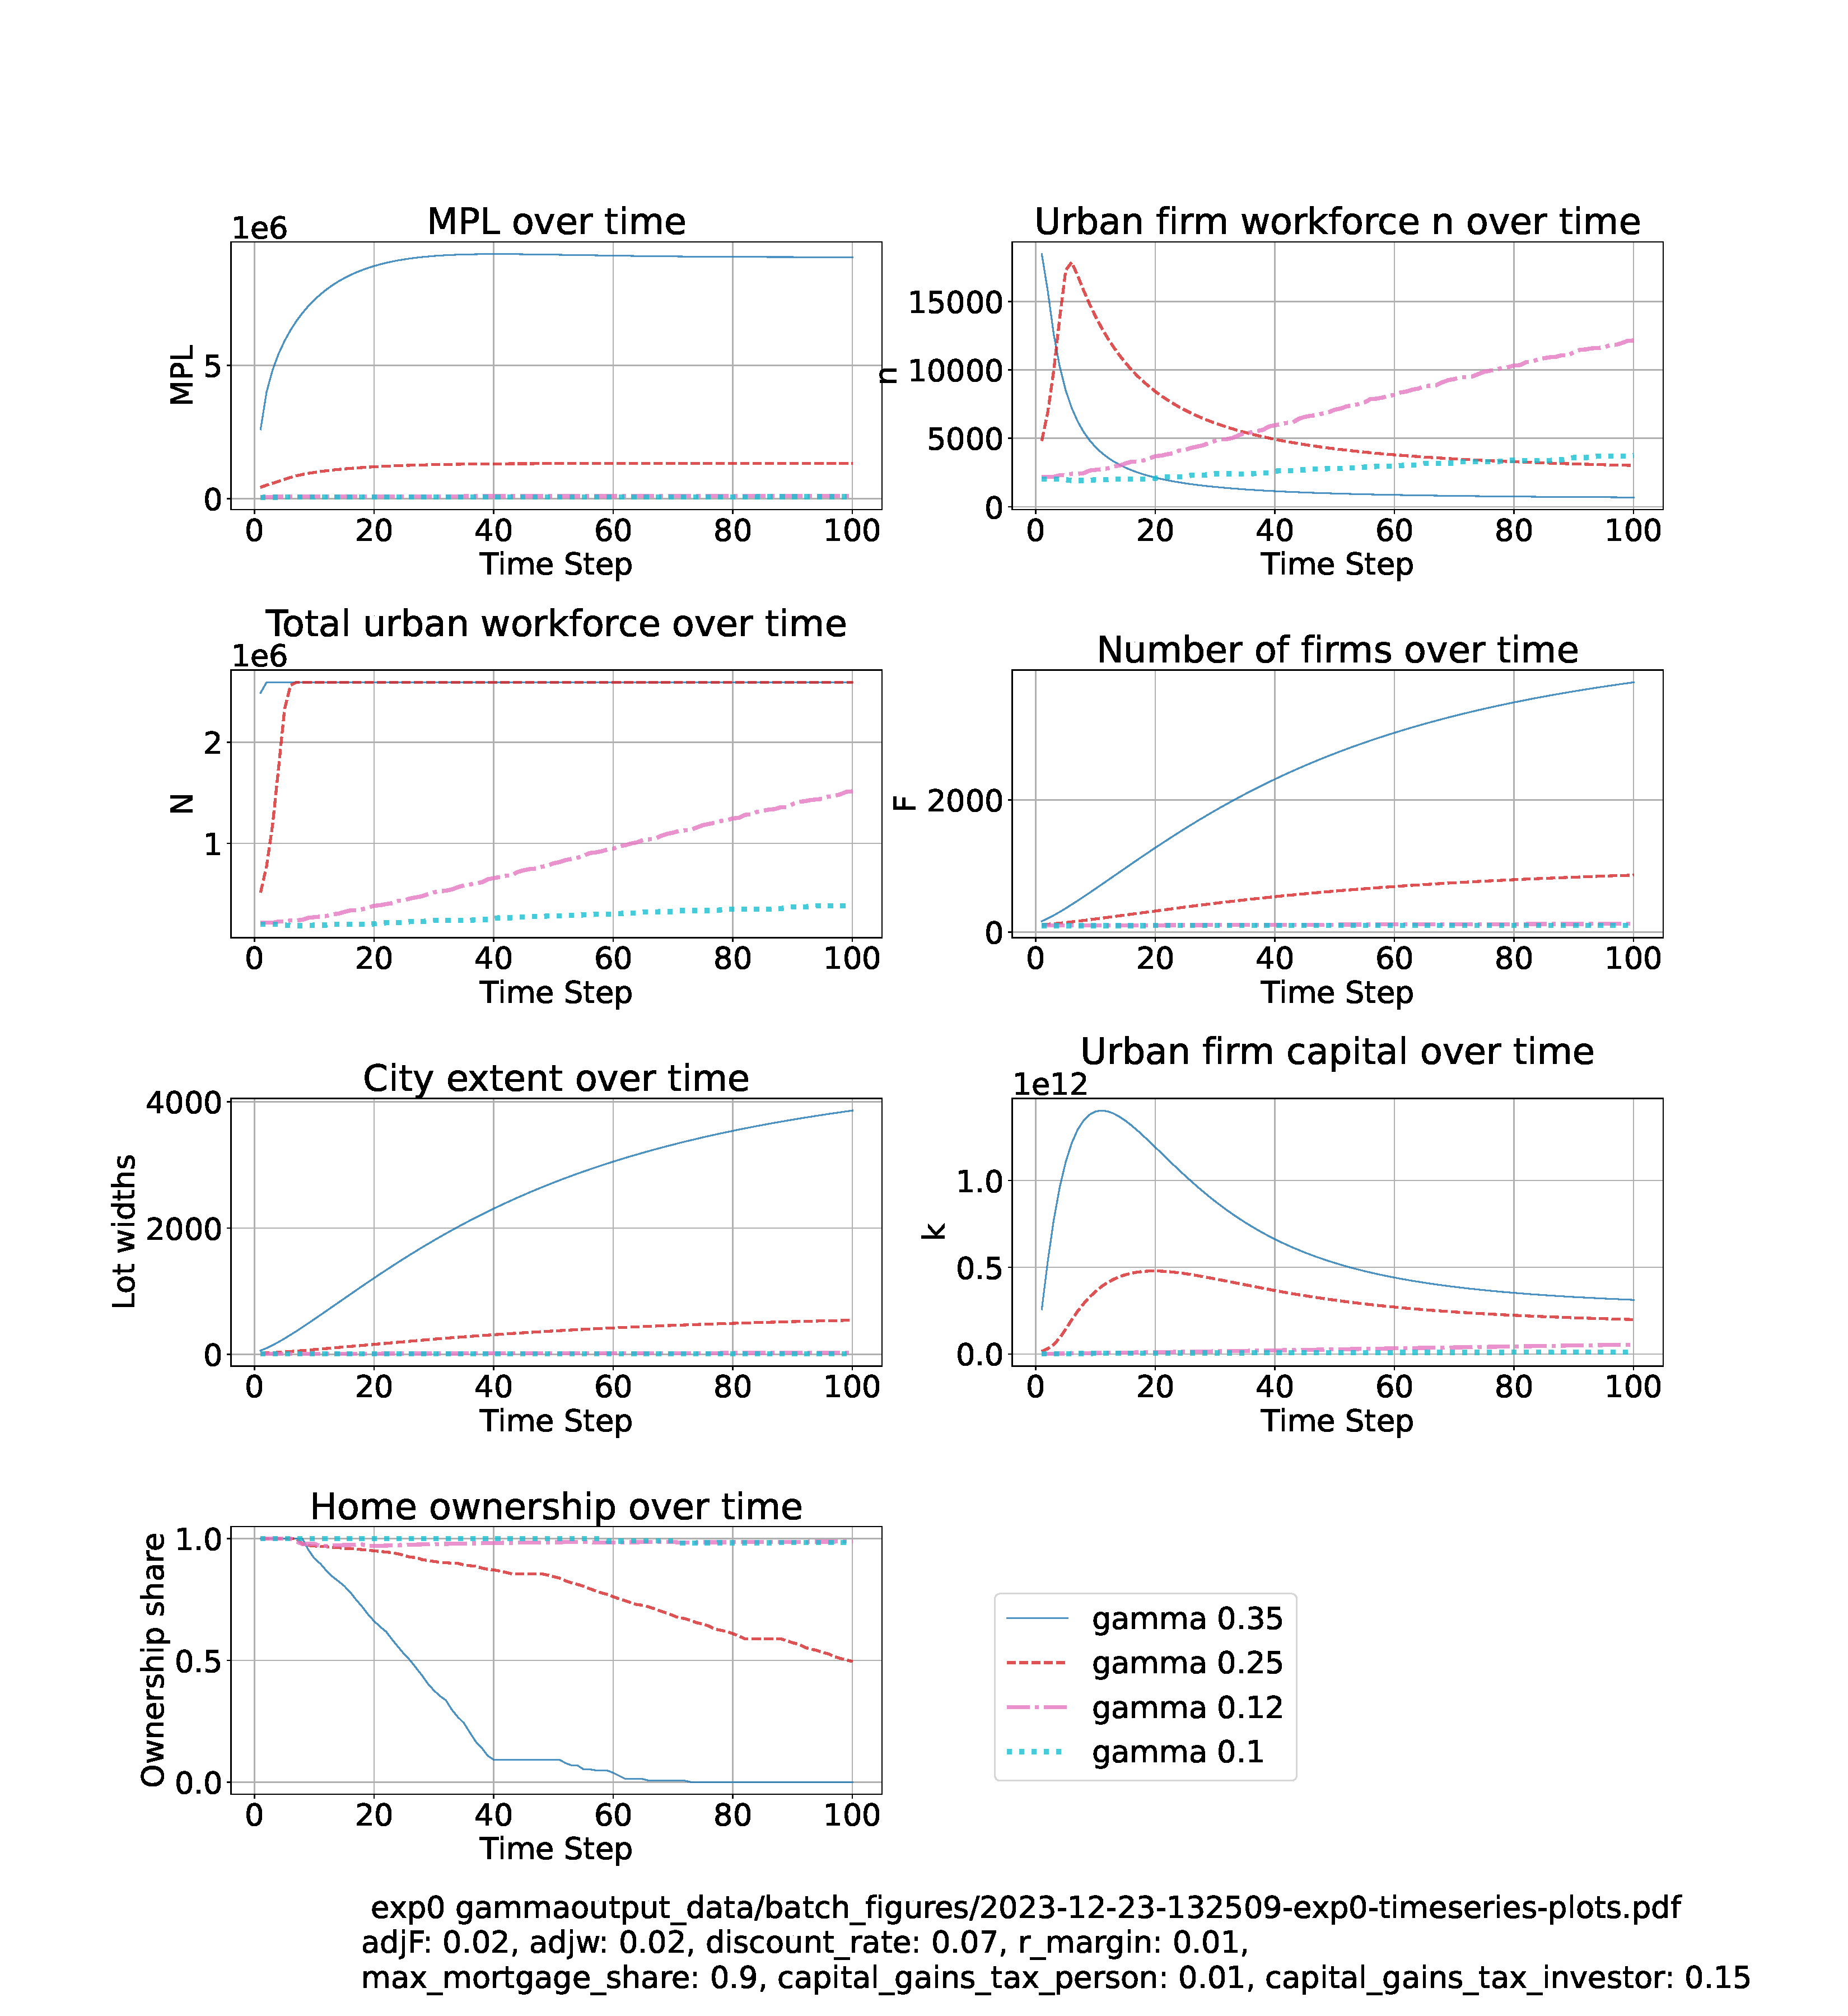
\includegraphics[trim= 1.5cm 3.65cm 2cm 4.0cm, clip, scale=.28]{fig/Analysis/Gamma-5-30.pdf}
